


\documentclass[runningheads]{llncs}
\usepackage[T1]{fontenc}
\usepackage{graphicx}
\usepackage{hyperref}
\usepackage{booktabs}
\usepackage{natbib}

\bibliographystyle{dinat}

\begin{document}


\title{
    The Evolution of Socks
}

\author{Dr. Cotton Weave\inst{ 1 }\orcidID{ 0000-1111-2222-3333 } \and
Prof. Woolford Stitch\inst{ 2,3 }\orcidID{ 1111-2222-3333-4444 } \and
Dr. Nylon Threadington\inst{ 3 }\orcidID{ 2222-3333-4444-5555 }
}

\institute{
International Sock Research Institute, London, UK \\ \and
Textile Innovation Center, Milan, Italy \\
\email{ textile-research@tic.org } \\
\url{ http://www.textile-innovation-center.org } \and
Academy of Footwear Sciences, Paris, France \\
\email{ research@footwear-academy.fr, publications@footwear-academy.fr } \\}


\authorrunning{Weave, 
Stitch, 
and Threadington
}

\maketitle

\begin{abstract}
This paper explores the historical evolution of socks, from ancient foot wrappings to modern performance textiles. 
We analyze key material innovations, cultural influences, and the impact of technology on sock design.
Our research includes case studies on compression wear, moisture-wicking fibers, and sustainable manufacturing.


\keywords{
Sock history \and Textile evolution \and Footwear technology \and Sustainable fashion.
}
\end{abstract}

\section{Introduction}\label{sec:Introduction}



Socks have been an essential part of human attire for thousands of years, evolving from crude animal hide wrappings to high-tech synthetic blends. Their history reflects advancements in textile manufacturing, economic trends, and cultural shifts. This paper provides an overview of the historical development of socks, their societal importance, and their modern-day innovations. For those unaware, \autoref{fig:sock} provides an example of such attire.



\begin{figure}
\centering
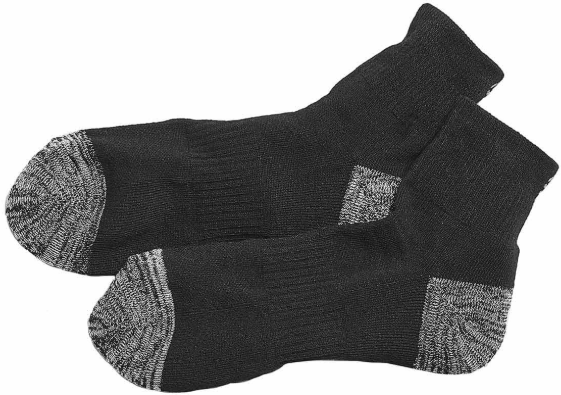
\includegraphics[width=0.4\textwidth]{/Users/ruipreis/Documents/Projects/obsitex/samples/sock-research-paper/images/sock.png}
\caption{Example of a sock}
\label{fig:sock}
\end{figure}


\section{Historical Evolution of Socks}\label{sec:Historical_Evolution_of_Socks}



Socks have undergone numerous transformations throughout history. Key developments include:



\begin{itemize}
	\item \textbf{Ancient} Origins: Early humans used animal skins and plant fibers to protect their feet from harsh environments.
	\item \textbf{Roman Era}: The Romans developed ‘udones,’ early knitted socks, signifying both practical use and social status.
	\item \textbf{Medieval Period}: Wool and silk socks became common among European aristocracy, often adorned with intricate embroidery \citep{acharBackPainChildren2020}.
	\item \textbf{Industrial Revolution}: The invention of knitting machines revolutionized sock production, making them widely accessible.
\end{itemize}




\section{Modern Innovations in Sock Manufacturing}\label{sec:Modern_Innovations_in_Sock_Manufacturing}



Recent advancements in sock technology include:



\begin{itemize}
	\item \textbf{Moisture-Wicking Fabrics}: Synthetic fibers enhance breathability and moisture control.
	\item \textbf{Compression Socks}: Designed for improved circulation, these socks are commonly used by athletes and medical patients \citep{weiFinetunedLanguageModels2022,aghajanyanIntrinsicDimensionalityExplains2020}.
	\item \textbf{Sustainable Materials}: Eco-friendly options like bamboo and recycled polyester reduce environmental impact \citep{acharBackPainChildren2020}.
\end{itemize}


\section{Socks Facts Table}\label{sec:Socks_Facts_Table}



\begin{table}
\centering
\caption{The Evolution of Socks - A Comparison of Historical and Modern Aspects}
\begin{tabular}{lrr}
\toprule
Feature & Historical Significance & Modern Relevance \\
\midrule
Material & Wool, silk, cotton & Bamboo, synthetics \\
First Use & Ancient Egypt (2500 BC) & Everyday essential \\
Fashion Trends & Aristocratic embroidery & Patterned, novelty socks \\
Medical Benefits & Foot protection & Compression therapy \\
Environmental Impact & Minimal (natural fibers) & High (synthetics) \\
\bottomrule
\end{tabular}
\end{table}



\bibliography{main}                         


\end{document}